\chapter{2D Wave numerical experiments}\label{sec:2d_numerical_experiments}
%------------------------------------------------------------------------------
\section{Gaussian hump}
In this section some numerical results are given for the
2D Gaussian hump.
The numerical tests are performed with some different time steps ($\Dt$), different space resolution (but with $\Dx=\Dy$) and different geometry, but all with the same constant bed level at $z_b = \bqty{-10}{\metre}$.
%--------------------------------------------------------------------------------
\subsection{Gaussian hump}\label{sec:num_exp_gaussian_hump}
The considered 2-D wave equation reads:
\begin{align}
    \pdiff{h}{t}  + \nabla \dotp \vec{q} & = 0 \qquad \textit{continuity eq.} \\
    \pdiff{q}{t}  + g h \nabla \zeta & = 0 \qquad \textit{momentum eq.}
\end{align}
%
With initial conditions
\begin{align}
    h(x,y,0) & = \zeta(x,y,0) - z_b(x,y), \quad \bunit{\metre} \\
    q(x,y,0) & = 0, \quad \bunit{\square\metre\per\second}
\end{align}
for the the water level a Gaussian hump is prescribed
\begin{align}
    \zeta(x,y) =  a_0 \exp\left[ -\left( \frac{(x - \mu_x)^2}{2\sigma^2_x} + \frac{(y - \mu_y)^2}{2\sigma^2_y}\right)\right], \quad \bunit{\metre}.
\end{align}
At the boundaries no ingoing signals are prescribed, so outgoing signals are leaving the domain unhampered, which means no reflections will be present other then numerical reflections.
%--------------------------------------------------------------------------------
\paragraph*{Numerical experiment}
The numerical experiment is performed with the following parameters:
\begin{itemize}
    \item Length of the domain, $L_x = L_y = \bqty{6000}{\metre}$, ranging from $\bqty{-3000}{\metre}$ to $\bqty{3000}{\metre}$.
    \item Bed level, $z_b = \bqty{-10}{\metre}$.
    \item Grid size, $\Dx = \Dy = \bqty{10}{\metre}$.
    \item Start time, $t_{start} = \bqty{0}{\second}$.
    \item End time, $t_{stop} = \bqty{1800}{\second}$.
    \item Timestep, $\Dt = \bqty{10}{\second}$.
    \item Amplitude of the Gaussian hump, $a_0 = \bqty{0.01}{\metre}$.
    \item Centre of the Gaussian hump, $\mu_x = \mu_y = \bqty{0}{\metre}$.
    \item Spreading of the Gaussian hump, $\sigma_x = \sigma_y = \bqty{350}{\metre}$.
\end{itemize}

%--------------------------------------------------------------------------------
\paragraph*{Results of the numerical experiments 1}
\notyet
%--------------------------------------------------------------------------------
\subsection{Gaussian hump, reflection}\label{sec:gaussian_hump_refelction}
The Gaussian hump test case is used to determine the reflection of a wave at the boundary. The schematization for this test is shown in \autoref{fig:two_mesh_reflection}.
\begin{figure}[H]
    \centering
    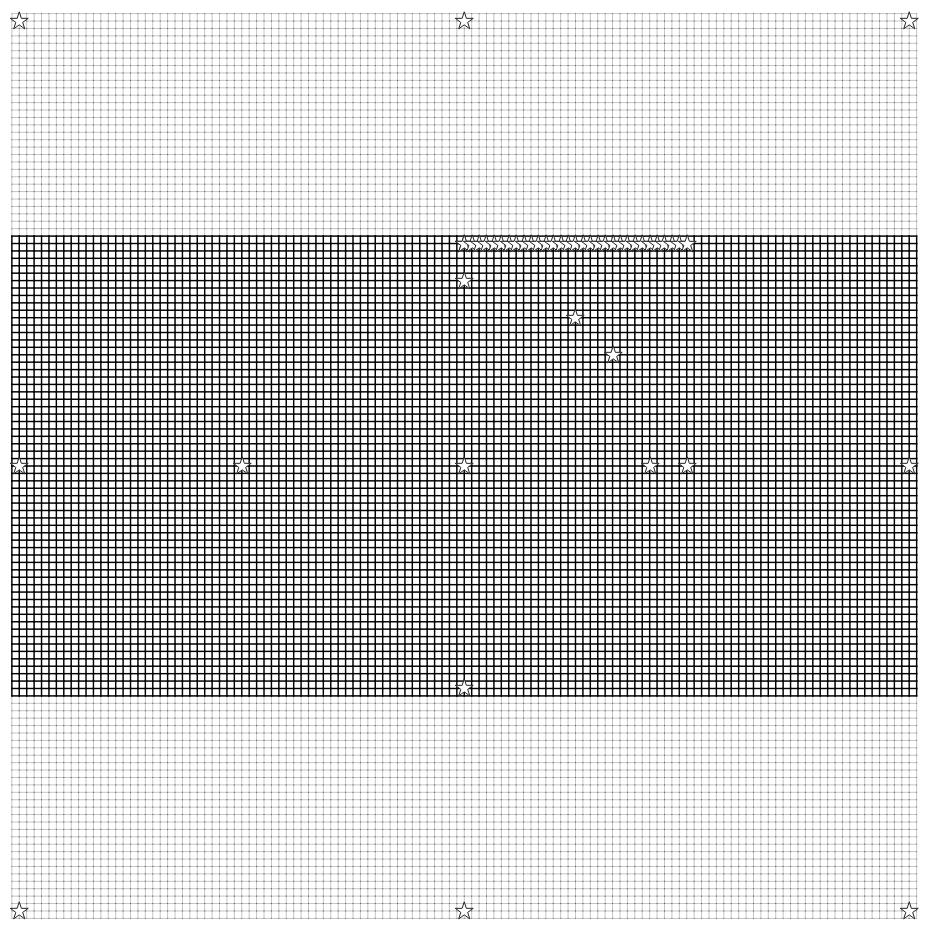
\includegraphics[width=0.9\textwidth]{figures/two_meshes_for_reflection.png}
    \caption{Schematization area: \emph{[-6000,6000]x[-6000, 6000]} \bunit{m} and \emph{[-6000, 6000]x\newline [-3000, 3000]} \bunit{\metre}. The observation points at $y=\bqty{3000}{\metre}$ are present on both meshes and are used to determine the refelection of a wave at these location}\label{fig:two_mesh_reflection}
\end{figure}

\notyet